\documentclass[tikz,border=10pt]{standalone}

\usepackage{amsmath,amssymb}
\usepackage{tikz}
\usetikzlibrary{arrows.meta,positioning,calc,fit}

\newcommand{\F}{\mathbb{F}}
\newcommand{\C}{\mathbb{C}}
\newcommand{\Z}{\mathbb{Z}}
\newcommand{\Spec}{\operatorname{Spec}}

\begin{document}
	
	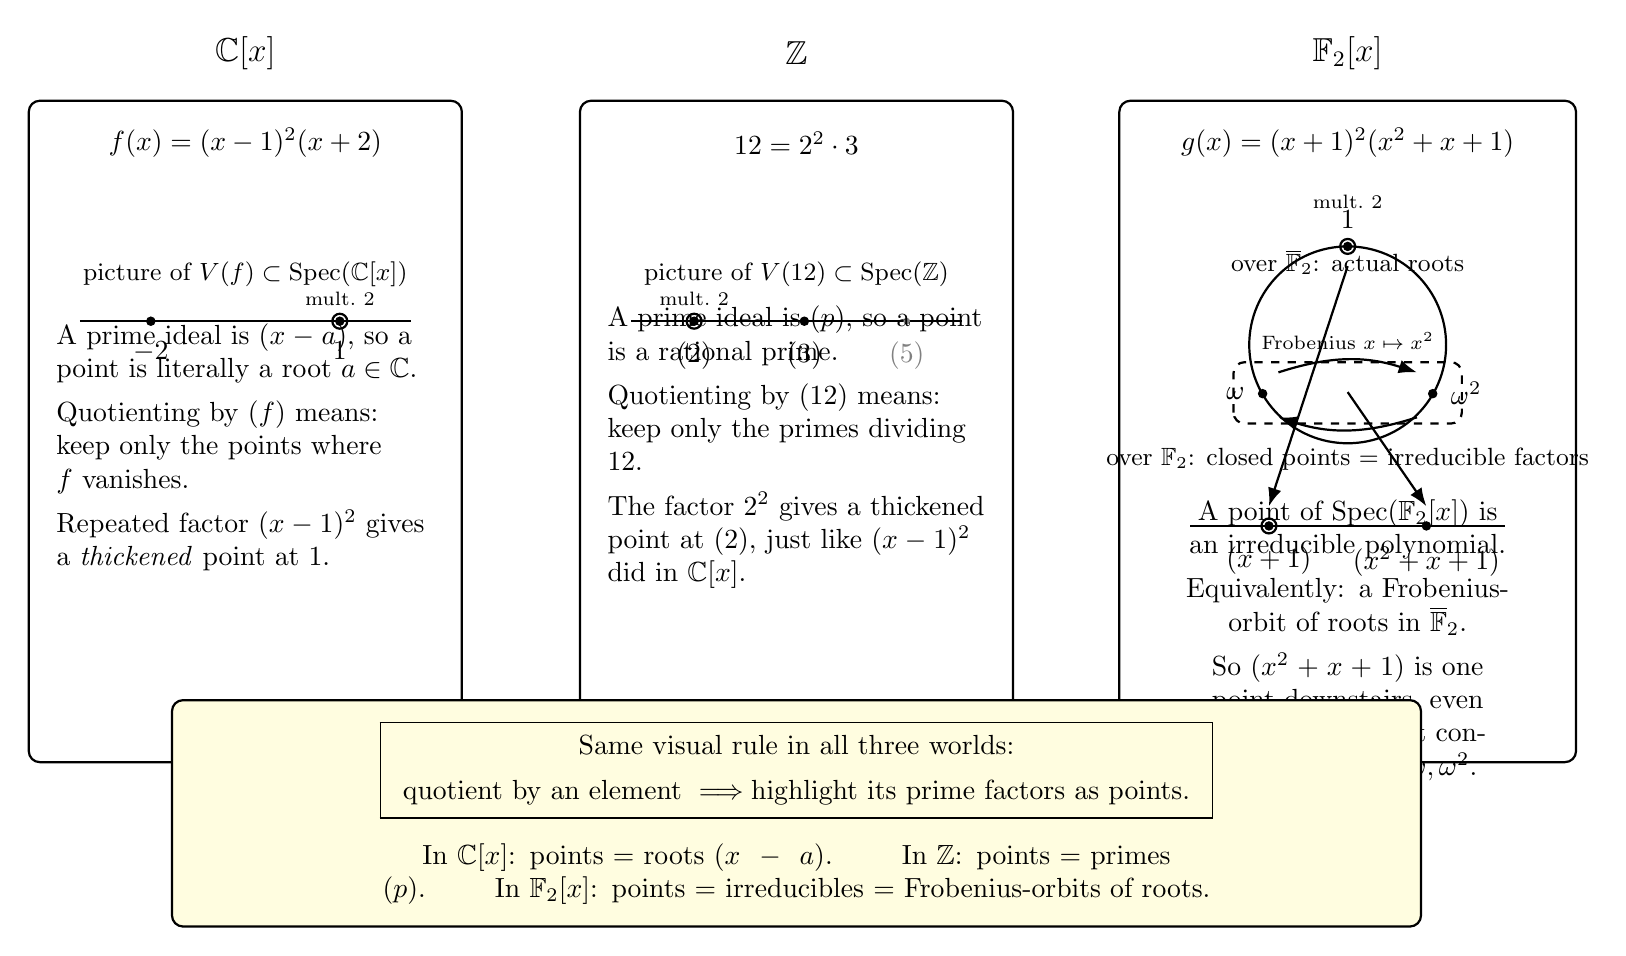
\begin{tikzpicture}[
		>=Latex,
		panel/.style={draw, rounded corners, thick, inner sep=8pt},
		title/.style={font=\bfseries\large},
		note/.style={align=left, text width=4.8cm},
		smallnote/.style={align=center, text width=4.3cm},
		orbit/.style={draw, dashed, rounded corners, thick}
		]
		
		% --------------------------------------------------
		% Titles
		% --------------------------------------------------
		\node[title] at (-7,5.2) {$\C[x]$};
		\node[title] at (0,5.2) {$\Z$};
		\node[title] at (7,5.2) {$\F_2[x]$};
		
		% --------------------------------------------------
		% LEFT PANEL: C[x]
		% --------------------------------------------------
		\node[panel, minimum width=5.5cm, minimum height=8.4cm] (L) at (-7,0.4) {};
		
		\node at ($(L.north)+(0,-0.55)$) {$f(x)=(x-1)^2(x+2)$};
		
		% affine line
		\draw[thick] ($(L.center)+(-2.1,1.4)$) -- ($(L.center)+(2.1,1.4)$);
		\node[below] at ($(L.center)+(-2.1,1.4)$) {};
		\node at ($(L.center)+(0,2.0)$) {\small picture of $V(f)\subset \Spec(\C[x])$};
		
		% points
		\filldraw[black] ($(L.center)+(-1.2,1.4)$) circle (1.5pt);
		\node[below=4pt] at ($(L.center)+(-1.2,1.4)$) {$-2$};
		
		\draw[thick] ($(L.center)+(1.2,1.4)$) circle (2.7pt);
		\filldraw[black] ($(L.center)+(1.2,1.4)$) circle (1.5pt);
		\node[below=4pt] at ($(L.center)+(1.2,1.4)$) {$1$};
		\node[above=2pt] at ($(L.center)+(1.2,1.4)$) {\scriptsize mult.\ $2$};
		
		\node[note] at ($(L.center)+(0,-0.2)$) {%
			A prime ideal is \((x-a)\), so a point is literally a root \(a\in\C\).\\[4pt]
			Quotienting by \((f)\) means: keep only the points where \(f\) vanishes.\\[4pt]
			Repeated factor \((x-1)^2\) gives a \emph{thickened} point at \(1\).
		};
		
		% --------------------------------------------------
		% MIDDLE PANEL: Z
		% --------------------------------------------------
		\node[panel, minimum width=5.5cm, minimum height=8.4cm] (M) at (0,0.4) {};
		
		\node at ($(M.north)+(0,-0.55)$) {$12=2^2\cdot 3$};
		
		% arithmetic line of primes
		\draw[thick] ($(M.center)+(-2.1,1.4)$) -- ($(M.center)+(2.1,1.4)$);
		\node at ($(M.center)+(0,2.0)$) {\small picture of $V(12)\subset \Spec(\Z)$};
		
		\filldraw[black] ($(M.center)+(-1.3,1.4)$) circle (1.5pt);
		\node[below=4pt] at ($(M.center)+(-1.3,1.4)$) {$(2)$};
		\draw[thick] ($(M.center)+(-1.3,1.4)$) circle (2.7pt);
		\node[above=2pt] at ($(M.center)+(-1.3,1.4)$) {\scriptsize mult.\ $2$};
		
		\filldraw[black] ($(M.center)+(0.1,1.4)$) circle (1.5pt);
		\node[below=4pt] at ($(M.center)+(0.1,1.4)$) {$(3)$};
		
		\filldraw[gray] ($(M.center)+(1.4,1.4)$) circle (1pt);
		\node[below=4pt, gray] at ($(M.center)+(1.4,1.4)$) {$(5)$};
		
		\node[note] at ($(M.center)+(0,-0.2)$) {%
			A prime ideal is \((p)\), so a point is a rational prime.\\[4pt]
			Quotienting by \((12)\) means: keep only the primes dividing \(12\).\\[4pt]
			The factor \(2^2\) gives a thickened point at \((2)\), just like \((x-1)^2\) did in \(\C[x]\).
		};
		
		% --------------------------------------------------
		% RIGHT PANEL: F2[x]
		% --------------------------------------------------
		\node[panel, minimum width=5.8cm, minimum height=8.4cm] (R) at (7,0.4) {};
		
		\node at ($(R.north)+(0,-0.55)$) {$g(x)=(x+1)^2(x^2+x+1)$};
		
		% top: geometric roots over algebraic closure
		\node at ($(R.center)+(0,2.15)$) {\small over $\overline{\F}_2$: actual roots};
		\draw[thick] ($(R.center)+(0,1.1)$) circle (1.25cm);
		
		\filldraw[black] ($(R.center)+(0,2.35)$) circle (1.5pt);
		\node[above=3pt] at ($(R.center)+(0,2.35)$) {$1$};
		\draw[thick] ($(R.center)+(0,2.35)$) circle (2.7pt);
		\node[above=10pt] at ($(R.center)+(0,2.35)$) {\scriptsize mult.\ $2$};
		
		\filldraw[black] ($(R.center)+(-1.08,0.48)$) circle (1.5pt);
		\node[left=3pt] at ($(R.center)+(-1.08,0.48)$) {$\omega$};
		
		\filldraw[black] ($(R.center)+(1.08,0.48)$) circle (1.5pt);
		\node[right=3pt] at ($(R.center)+(1.08,0.48)$) {$\omega^2$};
		
		\draw[->, thick] ($(R.center)+(-0.88,0.75)$) to[bend left=18] node[above] {\scriptsize Frobenius $x\mapsto x^2$} ($(R.center)+(0.88,0.75)$);
		\draw[->, thick] ($(R.center)+(0.88,0.18)$) to[bend left=18] ($(R.center)+(-0.88,0.18)$);
		
		\draw[orbit] ($(R.center)+(-1.45,0.1)$) rectangle ($(R.center)+(1.45,0.88)$);
		
		% bottom: closed points over F2
		\node at ($(R.center)+(0,-0.35)$) {\small over $\F_2$: closed points = irreducible factors};
		
		\draw[thick] ($(R.center)+(-2.0,-1.2)$) -- ($(R.center)+(2.0,-1.2)$);
		
		\filldraw[black] ($(R.center)+(-1.0,-1.2)$) circle (1.5pt);
		\node[below=4pt] at ($(R.center)+(-1.0,-1.2)$) {$(x+1)$};
		\draw[thick] ($(R.center)+(-1.0,-1.2)$) circle (2.7pt);
		
		\filldraw[black] ($(R.center)+(1.0,-1.2)$) circle (1.5pt);
		\node[below=4pt] at ($(R.center)+(1.0,-1.2)$) {$(x^2+x+1)$};
		
		\draw[->, thick] ($(R.center)+(0,2.1)$) -- ($(R.center)+(-1.0,-0.95)$);
		\draw[->, thick] ($(R.center)+(0,0.5)$) -- ($(R.center)+(1.0,-0.95)$);
		
		\node[smallnote] at ($(R.center)+(0,-2.65)$) {%
			A point of $\Spec(\F_2[x])$ is an irreducible polynomial.\\[4pt]
			Equivalently: a Frobenius-orbit of roots in $\overline{\F}_2$.\\[4pt]
			So \((x^2+x+1)\) is one point downstairs, even though upstairs it contains two roots \(\omega,\omega^2\).
		};
		
		% --------------------------------------------------
		% Bottom master rule
		% --------------------------------------------------
		\node[
		draw,
		rounded corners,
		thick,
		fill=yellow!12,
		text width=15.3cm,
		align=center,
		inner sep=8pt
		] (S) at (0,-4.45) {%
			$\boxed{
				\begin{array}{c}
					\text{Same visual rule in all three worlds:} \\[4pt]
					\text{quotient by an element } \Longrightarrow \text{highlight its prime factors as points.}
				\end{array}
			}$\\[8pt]
			In \(\C[x]\): points \(=\) roots \((x-a)\). \qquad
			In \(\Z\): points \(=\) primes \((p)\). \qquad
			In \(\F_2[x]\): points \(=\) irreducibles \(=\) Frobenius-orbits of roots.
		};
		
	\end{tikzpicture}
	
\end{document}